
\begin{figure}
\begin{verbatim}
library(SummarizedExperiment)
library(BiocOncoTK)
library(ggplot2)
cdar = BiocOncoTK::darmGBMcls
ind = match("PTPRC", rowData(cdar)$symbol)
var = gsub("selection: ", "", 
       cdar$characteristics_ch1.8)
vals = log10(as.numeric(assay(cdar[ind,])+1))
ddd = data.frame(log10norm=vals, pan=var)
ggplot(ddd, aes(x=log10norm, colour=pan)) + 
  geom_density() + ylim(0,1) + 
  xlab("log10 CD45+1")
\end{verbatim}
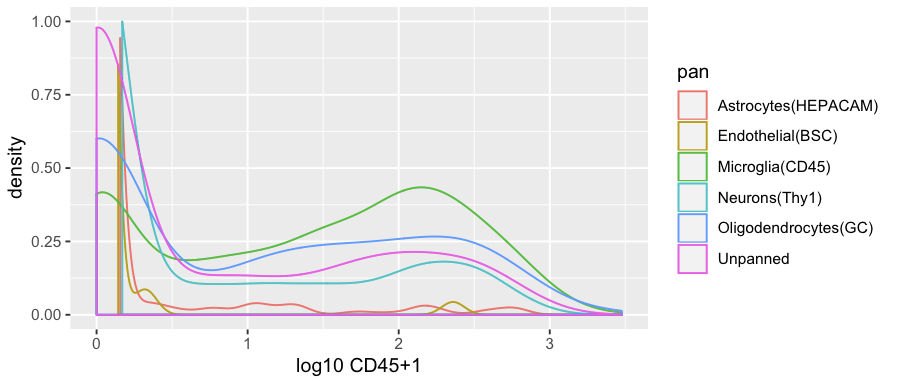
\includegraphics[height=4.0cm]{darmDens.png}
\caption{Code and density displays for
distribution of PTPRC (HGNC symbol for CD45) across immunopanned
cells reported in \cite{Darmanis2017}.
\texttt{BiocOncoTK::darmGBMcls} includes
a reference to HDF Cloud representation of
this glioblastoma single-cell RNA-seq
as requantified in the CONQUER project \citep{Soneson2018}.}
\label{hdffig}
\end{figure}

